% This is samplepaper.tex, a sample chapter demonstrating the
% LLNCS macro package for Springer Computer Science proceedings;
% Version 2.20 of 2017/10/04
%
\documentclass[runningheads]{llncs}
%
\usepackage{float}
\usepackage{graphicx}
\usepackage{makecell}
\usepackage{amsmath}
\usepackage{amssymb}
\usepackage{caption}
\newcommand{\trishita}[1]{}%{{\color{magenta}\bfseries[Trishita: #1]}}
\newenvironment{claimproof}[1]{\par\noindent\underline{Proof:}\space#1}{\hfill $\blacksquare$}

% Used for displaying a sample figure. If possible, figure files should
% be included in EPS format.
%
% If you use the hyperref package, please uncomment the following line
% to display URLs in blue roman font according to Springer's eBook style:
% \renewcommand\UrlFont{\color{blue}\rmfamily}
\begin{document}
%
\title{Distributed Web Mining of Ethereum
}
\author{
Trishita Tiwari
\and
David Starobinski
\and
Ari Trachtenberg
}
%
\authorrunning{T. Tiwari et al.}
% First names are abbreviated in the running head.
% If there are more than two authors, 'et al.' is used.
%
\institute{Boston University, Department of Electrical and Computer Engineering, Boston, MA 02215, USA \\
\email{\{trtiwari,staro,trachten\}@bu.edu}}
%
\maketitle             
%
\begin{abstract}
We consider the problem of mining crytocurrencies by harnessing the inherent distribution capabilities of the World Wide Web. More specifically, we propose, analyze, and implement \verb|WebEth|, a browser-based distributed miner of the Ethereum cryptocurrency. \verb|WebEth| handles Proof-of-Work (PoW) calculations through individualized code that runs on the client browsers, and thereafter collates them at a web server to complete the mining operation. \verb|WebEth| is based on a lazy evaluation technique designed to function within the expected limitations of the clients, including bounds on memory, computation and communication bandwidth to the server. We provide proofs-of-concept of \verb|WebEth| based on \verb|JavaScript| and \verb|WebAssembly| implementations, with the latter reaching hash rates up to roughly 40~kiloHashes per second, which is only 30\% slower than the corresponding native \verb|C++|-based implementation.
Finally, we explore several applications of \verb|WebEth|, including monetization of web content, rate limitation to server access, and private Ethereum networks. Though several distributed web-based cryptominers have appeared in the wild (for other currencies), either in malware or in commercial trials, we believe that \verb|WebEth| is the first open-source cryptominer of this type.

\keywords{crypto-currency \and Ethereum \and distributed computing \and web-browser computing \and mining}
\end{abstract}
%
%
%
\section{Introduction}
Cryptocurrencies are increasingly gaining traction as a viable form of currency.  This has been accompanied by a correspondingly increasing interest in the efficient validation of cryptocurrency transactions.  Whereas initial efforts in this domain have focused on creating dedicated hardware for this task ~\cite{asics}, more recent approaches have examined repurposing existing infrastructure. Indeed, one such class of efforts has focused on the use of client web browsers as a platform for distributed computing~\cite{Cushing}. The growing popularity of CoinHive~\cite{coinhive} is a case in point of the potential success of distributed in-browser cryptocurrency mining as a commercial (if malicious) enterprise. 

In this work, we propose \verb|WebEth|, a browser-based distributed miner for the popular Ethereum block chain~\cite{ethereum}. \verb|WebEth| tackles the challenge of achieving a profitable hash rate within a distributed ensemble of browsers under constrained memory, computation and network usage. Indeed, every browser needs to store a data structure of at least 1~GB in memory in order to mine Ethereum. Clearly, it is unfeasible to transfer this entire data structure every time a browser loads a web page. Instead, \verb|WebEth| employs a lazy approach to generate this data structure while mining. Through our experiments, we show that this approach takes at most five minutes to reach a steady state hash rate -- making it ideal for web applications where users spend time, such as gaming and video streaming. Our experiments also show that \verb|WebEth| yields a hashing rate of up to 40 kiloHashes/s, which, despite the overhead from running the algorithm in a browser, is only 30\% smaller than the performance of a corresponding miner running natively. 

The main contributions of this work are as follows:
\begin{itemize}
\item We propose \verb|WebEth| \cite{WebEth}, an open-source implementation of a distributed web-based Ethereum cryptominer in both \verb|JavaScript| and \verb|WebAssembly| that can operate under relatively resource constrained environments. Though miners for other currencies exist in the wild (e.g. CoinHive~\cite{coinhive}), they are all proprietary and closed-source.
\item We provide theoretical analysis and experimental evidence of the potential efficacy of the lazy approach adopted by \verb|WebEth| to achieve high hashing rates.
\item We propose a number of potential applications built upon \verb|WebEth|, including rate-limiting server access, usage tracking, and content monetization.
\end{itemize}

\paragraph{Related Work:}
Distribution of a common task is hardly a new concept~\cite{scheduling,parallel,orca}, but the growing popularity and efficiency of dynamic web content and client-side scripting languages like \verb|JavaScript| and \verb|WebAssembly|
have made web browsers an enticing implementation option~\cite{WebFlow,Duda,Cushing}.  Coinhive~\cite{coinhive} has
built into this environment a proprietary method for mining the Monero cryptocurrency, but this is often done on
the browsers of unsuspecting users.  A more ethical, open-sourced alternative, the Basic Attention Token~\cite{basicAttentionToken}, is an Ethereum-based ERC20 token~\cite{erc20} currently in development to be used in conjunction with the Brave browser~\cite{BraveBrowser} to generate ad revenue for website publishers by \emph{measuring a user's attention} on an advertisement. This platform promises to balance the ties between website users, publishers, and advertisers to ensure that users get only ads they would accept, advertisers pay for actual users (instead of click bots), and publishers actually get revenue instead of begging users to turn off their ad blockers.

\paragraph{Roadmap:}
The remainder of the paper is organized as follows. In Section \ref{sec:background} we cover the relevant background and related literature for our work.  In particular, we provide a self-contained description of Ethash, the Ethereum mining Proof-of-Work (PoW), and \verb|WebAssembly|, the language in which we implement an efficient miner. Section \ref{sec:webeth} describes \verb|WebEth|, including its lazy approach to distributing the Ethash PoW over numerous, resource-constrained browsers. This section also includes a performance analysis. We present the experimental results of our implementations in Section \ref{sec:results}. In Section \ref{sec:applications} we discuss several potential applications of our mining platform. We conclude in Section \ref{sec:conclusion}.  

\section{Background}
\label{sec:background}
\subsection{Cryptocurrencies: a general overview}
Most cryptocurrencies like Ethereum involve storing transactions in blocks, and the entire history of transactions is collated in a data structure known as a block chain. The block chain is managed by dedicated machines called \emph{client nodes}; where each client node typically stores the entire block chain. However, because each client node operates on its own copy of the block chain, the block chains on different nodes may go out of sync. Hence, there needs to be an accepted mechanism to decide the order in which new transaction blocks are appended to this block chain. 
For this, every time a new transaction takes place, the transaction is pooled together with all other transactions that have been broadcasted to the network, but haven't been added to the block chain yet. For most currencies, the data structure that stores these unconfirmed transactions is known as the \emph{mem pool}. A miner picks valid transactions from his mem pool and creates a new block out of these transactions. Once this happens, the goal of the miner is to have his/her block appended to the block chain, which is achieved through a process called \emph{mining}.
Mining involves a race amongst miners to solve a \emph{Proof-of-Work} (PoW) puzzle, which is usually an energy intensive computation. The winner of this race gets to have his block appended to the block chain. The winner also receives a payout, which acts as an incentive to mine. 

Ethereum uses Ethash as its PoW algorithm, which is explained in detail below.

\subsection{Ethereum Proof of Work}
Ethereum is a crypto-currency that was released in July 2015 by Vitalik Buterin, Gavin Wood and Jeffrey Wilcke. Ethereum uses the Ethash algorithm (derived from the Dagger and Hashimoto algorithms ~\cite{dagger-hashimoto}) for its PoW for mining blocks. Before we discuss how mining works with Ethash, we first establish basic terminology about the data structures involved in the PoW.

A \emph{block header} contains meta-data related to the transactions of the corresponding block, and it is provided as an input to the Ethash algorithm together with an integer \emph{nonce}.  The nonce is chosen in a brute-force fashion in order to hash, together with the block header, into a value that matches a specific pattern (based on a predefined \emph{difficulty threshold}). The process of finding an appropriate nonce for a given block is known as \emph{mining}.

Once a block has been mined, it is propagated to other client nodes so that they can update their copies of the block chain. However, before each client node does so, it must validate whether the miner is submitting a legitimate block -- i.e., check whether the miner genuinely solved the hash as claimed. This is easily done by putting the block header and nonce associated with the block through the Ethash algorithm and checking whether the output follows the pattern prescribed by the difficulty threshold.  \emph{Light weight} client nodes do not mine new blocks, but rather only verify whether any new block submitted by a miner is valid or not.  \emph{Full} client nodes, on the other hand, both mine and verify new blocks.

An \emph{epoch} is a unit of ``time'' that spans 30,000 blocks.  All of the data structures in Ethash (mentioned below) need a 256 bit \emph{seed}, which differs for every epoch. For the first epoch the seed is a Keccak-256~\cite{keccak} hash of a series of 32 bytes of zeros. For every other epoch it is always the Keccak-256 hash of the previous seed hash.  The seed for a particular epoch is used to compute a data structure known as the \emph{Cache}, which is an array of 4 byte integers \cite{Ethmining}. The Cache production process involves using the seed hash to first sequentially fill up the Cache, then performing two passes of the RandMemoHash algorithm~\cite{randmemohash} on top of it to get the final Cache value. 

Light weight clients may use this Cache for verifying hashes, while full node clients can use it to calculate a Directed Acyclic Graph (DAG) dataset, as described below.  A Ethereum \emph{Directed Acyclic Graph} is stored as a large byte array (around 1 GB in size on the private Ethereum Network used for our experiments) and has the following two attributes:
  \begin{enumerate}
  \item \emph{Node}: Each DAG node in this byte array spans 64 bytes, and node indices are therefore aligned at a 64 byte boundary.
  \item \emph{Page}: Each DAG page spans 2 nodes, however, page accesses are not aligned at a 2 node boundary. The mining process involves accessing some DAG pages and hashing them together with the block header and nonce.
  \end{enumerate}
Each node in the DAG is generated by combining data from 256 pseudo-randomly selected Cache nodes and hashing them together. This process is repeated to generate all nodes in the DAG. Finally, intermediate byte arrays used to store temporary results in the Ethash algorithm are known as \emph{Mix}es.

We must point out that as time goes on, mining Ethereum becomes more and more difficult, as the size of the Cache and DAG increases with every epoch. 

\begin{figure}[h]
\centering
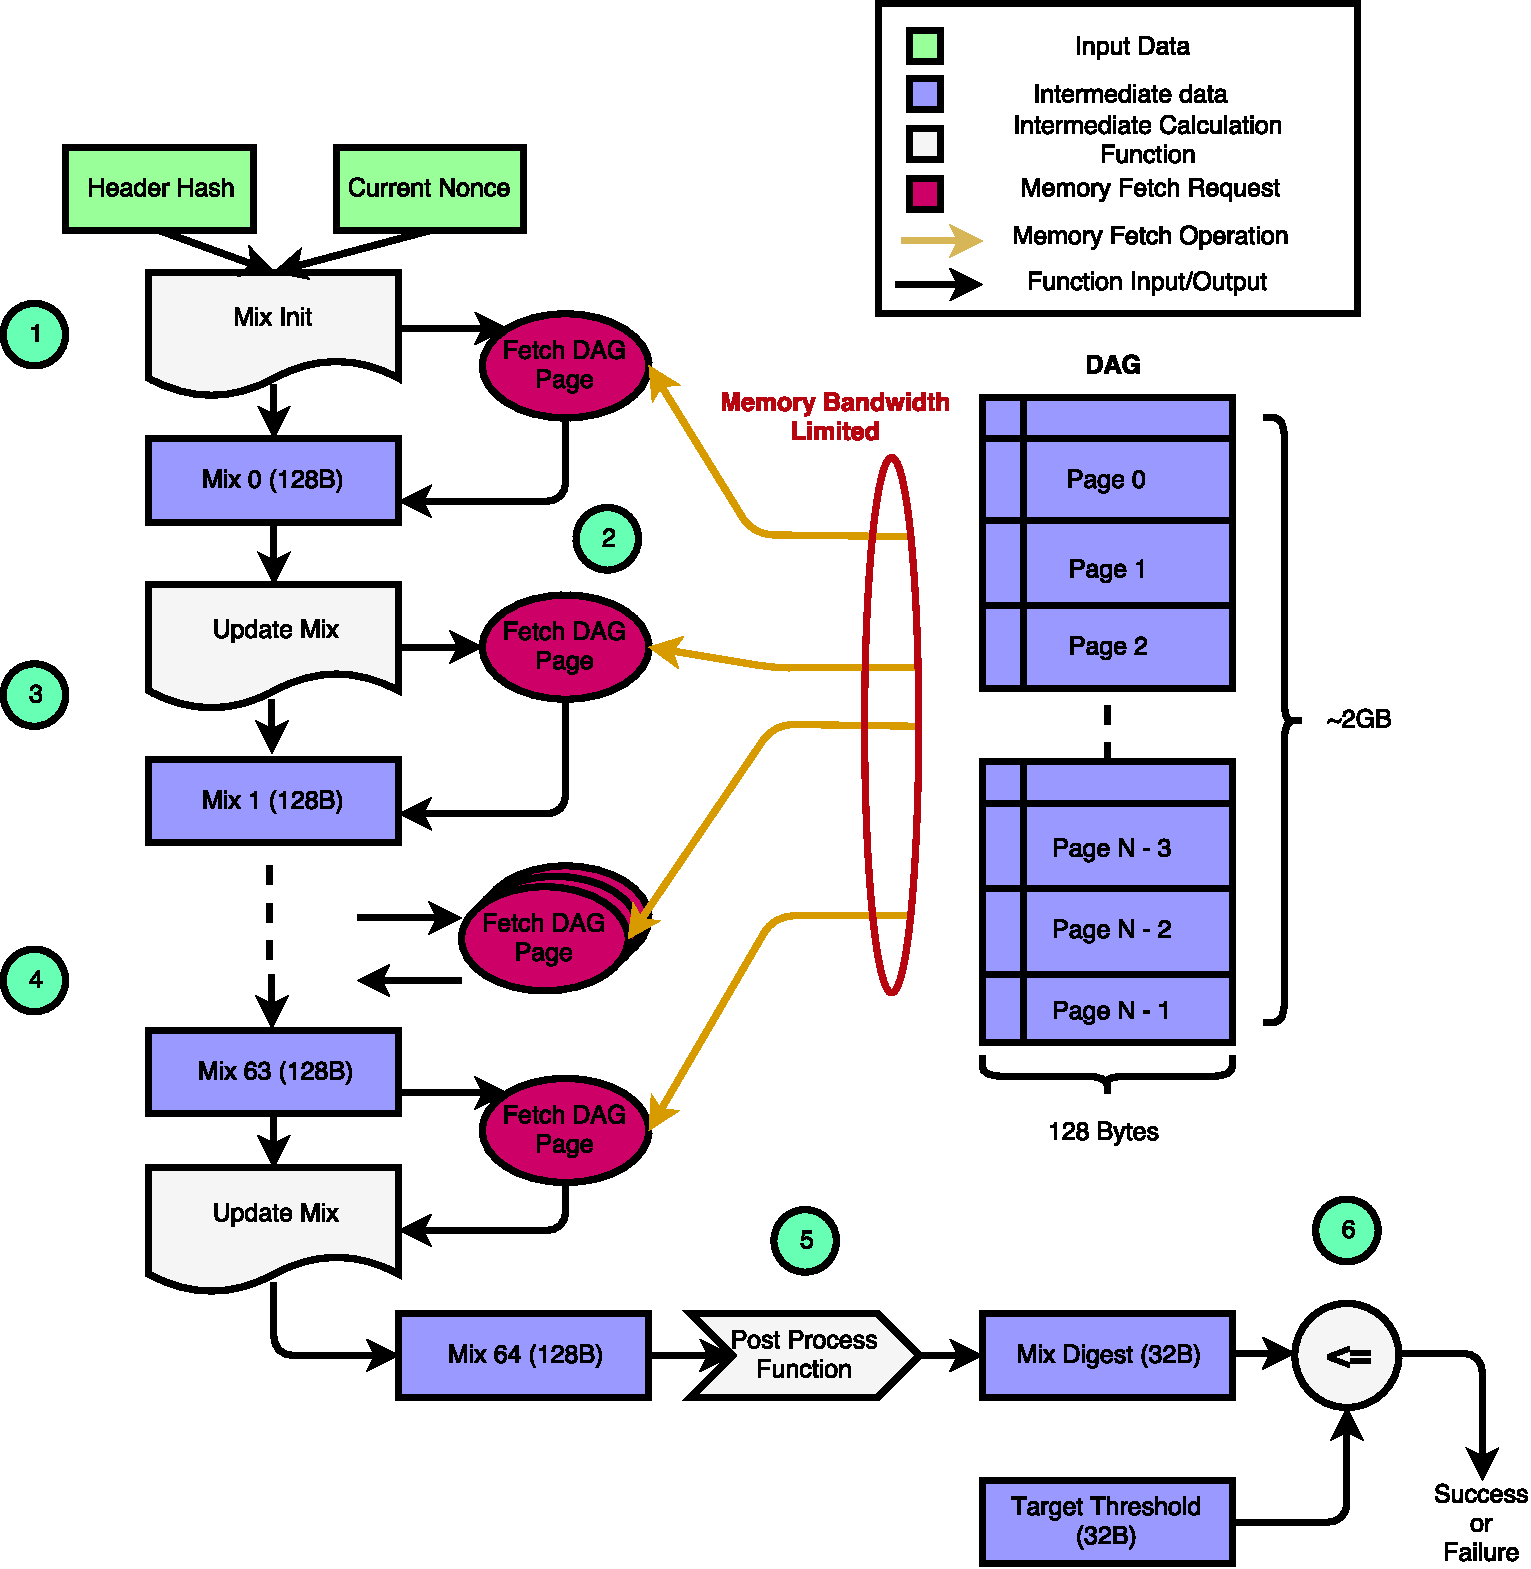
\includegraphics[width=300px,keepaspectratio]{Ethash.pdf}
\caption{Ethash}
\label{fig:ethash}
\end{figure}

Mining is performed by starting with the current block header hash and nonce, which are combined to get a 128-byte wide Mix, as seen in step 1 of Figure \ref{fig:ethash}. The Mix is then used to fetch a specific page of the DAG from memory. After this, the Mix is updated with the fetched page of the DAG (step 2). Then, this updated Mix is used to fetch a new page of the DAG (step 3). This process of sequentially fetching parts of the DAG is repeated 64 times (step 4), and the final value of the Mix is put through a transformation to obtain a 32 byte digest (step 5). This digest is then compared to the threshold (step 6). If it is smaller than the threshold, the nonce is valid and the block is successfully mined and can be broadcast to the network. However, if the digest is greater than the threshold, the nonce is unsuccessful, and the entire process must be repeated with a new nonce~\cite{Ethmining}. 


It is important to note that the pages of the DAG that are used to compute the hash for a particular block depend on the nonce used, hence there is no way to pre-determine which pages will be useful to have in memory. This therefore forces miners to store entire DAG in memory, making Ethereum mining ``Memory Hard''. 


Whereas mining is memory intensive, verification is relatively lightweight. This is because of the property that each node in the DAG depends on a set of pseudo-randomly selected items from the Cache. Hence, the Cache is used to regenerate only the specific pages of the DAG that are needed to recalculate the hash for the particular nonce. And so, only the Cache needs to be stored by light weight clients that only perform verification. In fact, as we will see in the next section, we use this property of being able to generate parts of the DAG as needed to our advantage in order to alleviate some of the memory and network bandwidth restrictions that browsers typically face.

\subsection{JavaScript and WebAssembly}
Introduced in 1995 by Netscape Communications Corporation~\cite{js}, \verb|JavaScript| was a meant to be a light scripting language in order to  make web content dynamic. Over the span of 23 years, it has grown to become one of the most popular client-side web development languages used to make dynamic user interfaces. 

In fact, up to recently, \verb|JavaScript| has been the only language available to make dynamic client-side web content. However, the situation has changed since the advent of \verb|WebAssembly| in 2016. As per its creators, \verb|WebAssembly| is a ``binary instruction format for a stack-based virtual machine'' \cite{webAssembly}. WASM is designed to be compiled from high-level languages like \verb|C/C++/Rust|, and is supported by 4 major browser platforms -- Firefox, Safari, IE, and Chrome \cite{webAssembly}. The \verb|WebAssembly| stack machine is designed to be encoded in a ``size-and load-time-efficient binary format''~\cite{webAssembly}, and aims to execute near native speed by utilizing common hardware capabilities present on a wide variety of platforms~\cite{webAssembly}. The language is meant to improve performance for computationally intensive use cases such as image/video editing, games, streaming, etc~\cite{webAssembly}. This makes it the language of choice to implement a miner within a browser. 

\section{WebEth}
\label{sec:webeth}
In this Section, we present our Web mining architecture for Ethereum. A diagram of the \verb|WebEth| architecture is depicted in Figure~\ref{fig:hybridArchitecture}. The architecture of the miner itself involves the browser connecting to a central node as soon as the web page loads (Steps 1 and 2 in Figure~\ref{fig:hybridArchitecture}). On connecting, the browser then receives the current block header hash and Cache (Step 3), using which it begins mining using the lazy evaluation algorithm discussed below (Step 4). Then, the browser could take one of two paths -- it could either have solved the block (Step 5a), in which case it sends the solution to the central node and asks for the next block to solve. Or it could timeout (Step 5b), in which case it polls the central node again for the current block header hash and Cache and then resumes mining. This architecture, including the lazy evaluation mining algorithm, is described in detail below.

\begin{figure}[h]
\centering
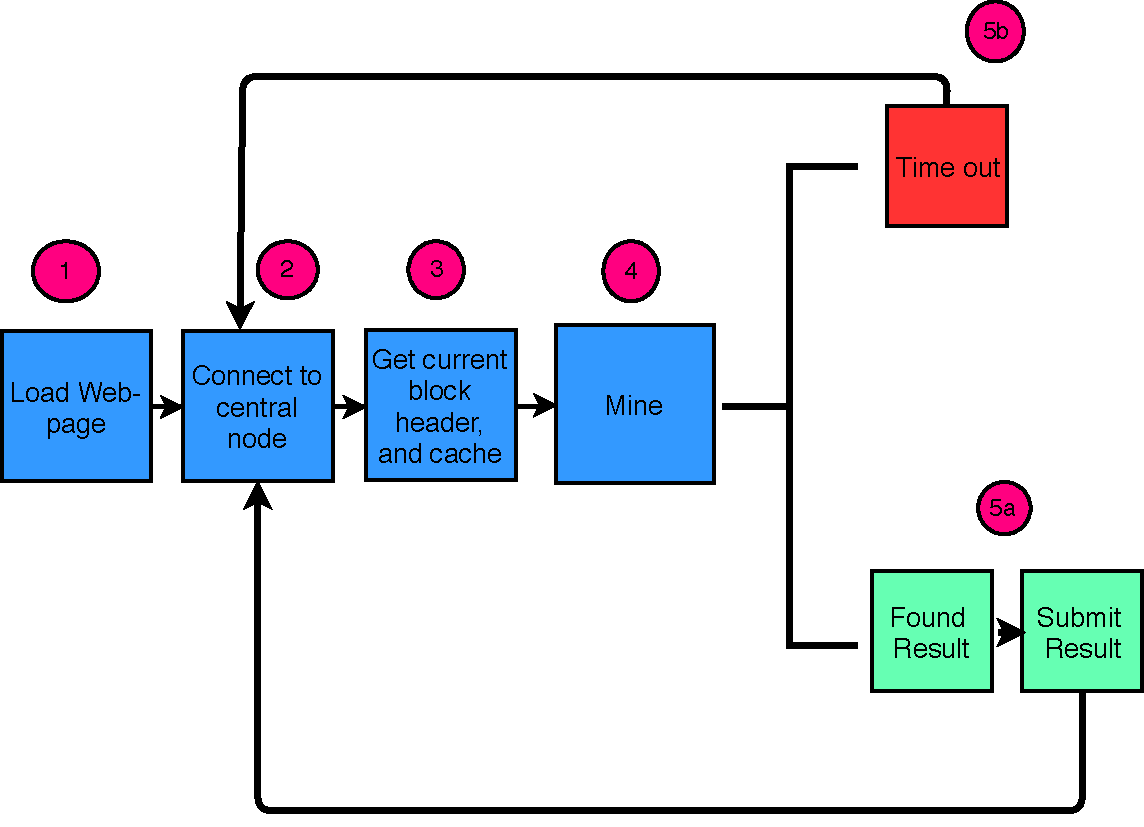
\includegraphics[width=230px,keepaspectratio]{Hybrid-Miner.pdf}
\caption{WebEth Architecture}
\label{fig:hybridArchitecture}
\end{figure}

\subsection{Lazy Evaluation}
The mining itself (Step 3) in \verb|WebEth| is based on a lazy evaluation to alleviate the network and memory requirements for mining Ethereum in a distributed scenario on browsers. Specifically, as soon as each browser connects to the webserver, the server sends to the browser the current block header hash and the Cache. Once the browser receives the Cache, it allocates an array buffer to store the DAG nodes.
 
Once the buffer is allocated, the browser can start iterating over nonces to compute hashes.  
Since, to begin with, the browser does not store any nodes of the DAG, it must compute each node on the fly using the Cache. However, every node that the browser computes is stored in the buffer, for quicker access in the future. Hence, as time passes, the buffer starts filling up, such that more and more nodes are quickly accessed from the buffer rather than being computed from the ground-up, which makes hash computations faster with time. This has the effect that the longer the user remains on the web-page, the better the hash rate gets for that user. 

\subsection{Implementation}

The \verb|WebEth| architecture is centered around a central node and client-side Ethereum miners. 

We have two implementation for the client-side miners: in \verb|JavaScript| and in \verb|WebAssembly|. For our miner, we model the \verb|JavaScript| implementation after the ~\verb|node.js| implementation of Ethash~\cite{ethash}. The \verb|WebAssembly| version is the \verb|JavaScript| version transpiled to \verb|C++|, which in turn is compiled to \verb|WebAssembly| using the ~\verb|Emscripten| compiler~\cite{emscripten}. 

The central node itself coordinates all workers (browsers). Its implementation is based on a modified version of \verb|geth| \cite{geth}, a real world Ethereum miner written in \verb|Go|. \verb|geth| typically runs as a standalone miner that mines on the machine on which it is running. We modify the code so that instead of doing all the mining all by itself, the node sends over the necessary data (namely, the hash of the Block Header and the Cache) to any client that connects to it on port \verb|9000| (Steps 1, 2 and 3 in Figure~\ref{fig:hybridArchitecture}). 

After receiving the necessary data, per the lazy evaluation algorithm, each browser allocates a buffer for the DAG in order to store future DAG nodes. (Note that the buffer for the DAG is implemented as an array of ints, so as to make each lookup in the buffer constant in time.) Now, the client-side miner can begin to mine (Step 4). 
At the beginning, the miner creates a random nonce and computes the hash (using the Cache and the buffered DAG) as discussed in the previous section. It continues to perform this action on new nonces until one of two following scenarios occur (Steps 5a and 5b). 

In the first scenario (Step 5a), the miner finds a nonce such that the computed hash is below the given threshold. In that case, the browser submits the result back to the central node and then asks the central node for the new block header hash and the Cache. It then uses these new inputs and continues to mine.

In the second scenario (Step 5b), the algorithm times out without finding a result. In that case, the miner polls the central node for the current versions of the block header hash and Cache and continues to mine using the new inputs. This process continue until the user moves away from the website or closes the browser. 
This time out is necessary since the browser should work with the most recent block header and Cache. The block header can become stale if that particular block has already been mined, and the Cache can become stale if the Ethereum network transitions into a new epoch (this happens once every 30,000 blocks). 

Finally, we must point out that both our current implementations in \verb|JavaScript| and \verb|WebAssembly| require no external dependencies, and therefore can be directly embedded into any website. Furthermore, the fact that the central server does not have to keep track of each client makes the system quite scalable. 

\subsection{Performance Analysis}
In this section, we perform a back-of-the envelope calculation for the number of hashes needed till \verb|WebEth| fills up almost all the buffer. This is important because the hash rate reaches its maximum steady-state only once the buffer in the browser is almost full. Specifically, we show that filling a buffer the size of the DAG till only $5*10^{-7}\%$ of it is empty should take on average about 1.85 million hashes,
% 3.7 million hashes, 
while filling it up till $5*10^{-1}\%$ of this buffer is empty takes much lesser -- about 700 thousand hashes.
% 1.4 million hashes. 
The approach we take is based on the Coupon Collector problem~\cite{couponCollector}. 

For simplicity, we assume that 128 nodes in the DAG are \textit{randomly} sampled in order to compute each hash, whereas, in reality, this is not entirely true. This is because Ethash samples 128 \textit{pages} per hash (rather than 128 \textit{nodes}). Since each page is two nodes wide, two \textit{neighboring} DAG nodes are sampled for each page computation. Hence, the DAG nodes are not accessed completely randomly. Nonetheless, this estimation still provides us a good approximation.
% Hence, in order to account for this simplification we also assume that 64 DAG \textbf{nodes} are used for each hash computation instead of 64 \textbf{pages} (or 128 nodes), and so our results suggest that it should take more hashes to fill the buffer up than it would in real life.
% For simplicity, we assume that the DAG is randomly sampled in order to compute hashes. In reality, this is not entirely true, because two neighboring DAG nodes are computed for each page computation (rather than a single node).  Hence, the results we obtain from the following analysis are more conservative than those observed in practice. 

For our analysis, we introduce the following notation. We denote by $N$ the total number of nodes in the DAG, by $a$ the number of DAG nodes needed to compute a hash, by $\delta$ the failure probability of finding a specific node in the buffer (i.e., the buffer miss rate), by $\omega$ the failure probability of computing a hash using nodes already stored in the buffer, by $E(X)$ the expected number of hashes to fill the buffer with a failure probability $\delta$, and by $H_n$ the $n$-th Harmonic number.
% ~\cite{harmonicNumber}.
\begin{claim}
For $\delta \ll 1$, $E(X) \approx \frac{N}{a}(H_{N} -H_{N\delta}).$
\end{claim}

\begin{claimproof}
The number of nodes needed in the buffer to achieve a failure probability $\delta$ is 
$\left \lceil{N(1-\delta)}\right \rceil$.
This means that even though we are allocating a buffer that can hold $N$ nodes, we are willing to forgo $\left \lfloor{N\delta}\right \rfloor$ nodes (to simplify notation, from now and on, we assume $N\delta$ is an integer).  

Using results from the Coupon Collector's problem~\cite{couponCollector}, we know that the expected number of trials for obtaining the $i$-th new node after having buffered $i-1$ nodes is $N/(N-(i-1))$.
Thus, the expected number of trials in order to fill up the buffer with ${N(1-\delta)}$ nodes is given by
\begin{gather}
	E(t) = N\sum_{i=1}^{N(1-\delta)} \frac{1}{N-i+1}.
\end{gather}
Splitting this expression into two sums, we get
\begin{gather}
	E(t) = N \left(\sum_{i=1}^{N}\frac{1}{N-i+1} - \sum_{i=N(1-\delta)+1}^{N}\frac{1}{N-i+1} \right), 
\end{gather}    
or
\begin{gather}
    \label{eq:expectedTrials}
    E(t) = N(H_{N} -H_{N\delta}).
\end{gather}
We now relate the failure probability  of calculating a hash using nodes already stored in the buffer  $\omega$ with the failure probability of having a specific node in the buffer $\delta$. By the independence assumption,
$$ 1-\omega = (1-\delta)^a$$For $\delta \ll 1$, we have $(1-\delta)^a \approx 1-a\delta$. Hence,
\begin{gather}
    \label{eq:deltaomega}
	\delta \approx \frac{\omega}{a}.
\end{gather}
Hence, it follows from Equation~(\ref{eq:deltaomega}) that 
\begin{gather}
	\label{eq:hashvspage}
	E(X) \approx \frac{E(t)}{a}.
\end{gather}
Finally, from Equations~(\ref{eq:expectedTrials}) and~(\ref{eq:hashvspage}) and, we obtain
\begin{gather}
    \label{eq:expectedHashes}
	E(X) \approx \frac{N}{a}(H_{N} -H_{N\delta}).
\end{gather}

\end{claimproof}

We use the following approximation on the Harmonic Numbers to compute  Equation~(\ref{eq:expectedHashes}):
\begin{gather}
    \label{eq:boundHarmonic}
    H_n \approx \ln{n} + \gamma + o(1)
\end{gather}

where $\gamma = 0.57721566...$ is the Euler-Mascheroni constant.

Specifically, using Equations~(\ref{eq:expectedHashes}) and~(\ref{eq:boundHarmonic}), and setting $N = 16777186$ (the number of nodes in the DAG for our experiments), $a = 128$ and $\delta = 5*10^{-9}$, we get $E(X) \approx 1.85$ million hashes. However, if we increase $\delta$ to $5*10^{-3}$, we get $E(X) \approx 700$ thousand hashes. Hence, we see that even computing merely 700 thousand hashes fills a DAG buffer as large as the entire DAG within a margin of $5*10^{-1}\%$, as opposed to calculating 1.85 million to fill it within a margin of $5*10^{-7}\%$. 
 
In fact, as we will see in the results, filling up 99.5\% of a buffer as large as the DAG already starts giving us good hash rates for a browser -- 35kH/s for the \verb|WebAssembly| miner. This shows that we need to have the buffer almost -- but not completely -- full in order to do well in terms of hash rates. And as we have seen, making the buffer almost full is not nearly as hard as filling it up entirely. 
This means that reaching a reasonably steady state is not as hard as it seems at face value, making \verb|WebEth| viable for web settings where users might not stay on websites for long. However, given this, we would also like to point out that in reality, while it takes a lot more hashes to fill up the buffer, it does not take a lot more \emph{time} to fill it up. This is because as discussed in the next section, when the buffer gets closer and closer to being full, the hash rate spikes up and so computing the remaining number of hashes to fill the buffer becomes quite fast. Hence, it does not take too long to completely fill up the buffer (around five minutes in our experimental setup), which is practical for many web applications, such as streaming.

\section{Results}
\label{sec:results}
\subsection{Experimental set up}
Our experimental set up consisted of a machine with an Intel i7-7700HQ processor with 8 cores and 16~GB ram. These results were obtained from a private Ethereum test network at epoch 0. The DAG size was 16777186 nodes (1.074~GB). The cache size was 1.677~MB. We ran the implementations in ~\verb|JavaScript| and ~\verb|WebAssembly| in the browser, and a native miner written in ~\verb|C++| that employs the same lazy evaluation approach outside of the browser for control results. Each miner was run till 800~kHashes were computed and the hash rate and buffer hit rate were sampled every 10k hashes. (Note that both the hash rate and buffer hit rate sampled at a particular time reflected the values over the 10k most recent hashes).

\subsection{Implementation Results}
Figures~\ref{fig:hashRateHMWASM}, \ref{fig:hashRateHMJS} and \ref{fig:hashRateHMNative} below shows a heat-map of how the hash rate varies for each of the three implementations as a function of both the size of the buffer allocated to store the DAG (as a percentage of the size of the entire DAG) and the number of hashes computed in the browser. Further, Figure \ref{fig:HitRateHM} then shows a heat-map of how the DAG buffer hit-rate varies as a function of both these parameters. 
As expected, both the hash rate and the buffer hit rate increases with the buffer size and the number of hashes computed for all three miners. We must also note that the experimental results suggest that it takes 700~kHashes to reach a buffer hit rate of 99.5\%, which agrees with our predicted value from the mathematical analysis in the previous section. In fact, we can validate that our experimental results are typically in agreement with the predicted results for all other hit rates as well.

\begin{figure}[h]
\centering
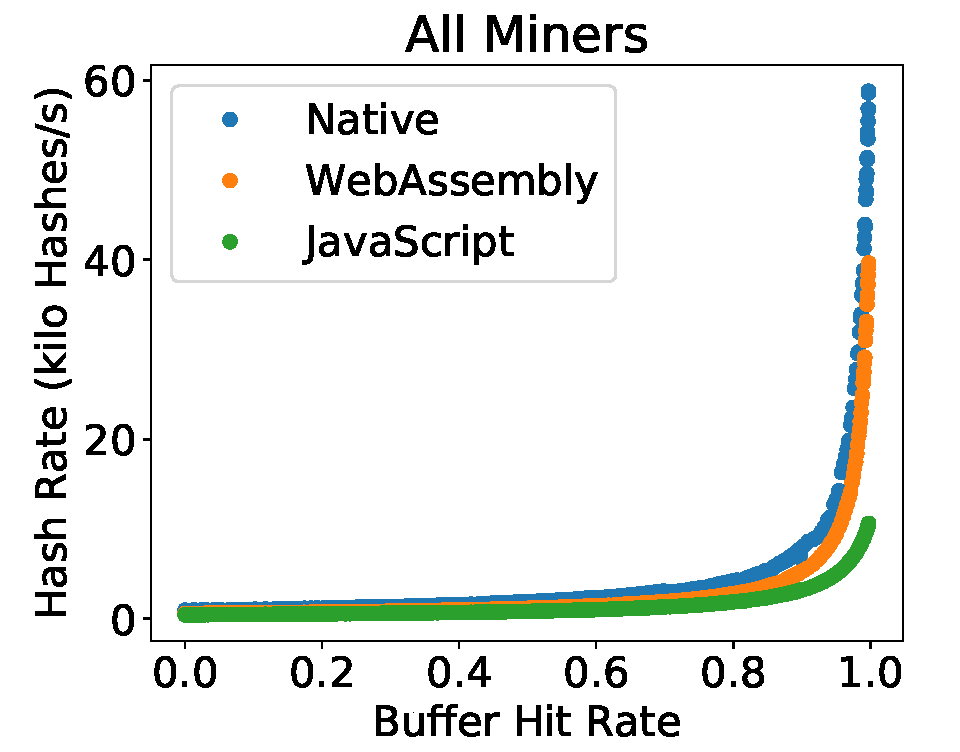
\includegraphics[width=200px,keepaspectratio]{All_Miners_Hash_Rate.pdf}
\caption{All Miners' Hash Rate}
\label{fig:HashRateTraj} 
\end{figure}

\begin{figure}[t]
       \centering
    \makebox[\textwidth][c]{
    \begin{minipage}{.5\textwidth}
       \centering
  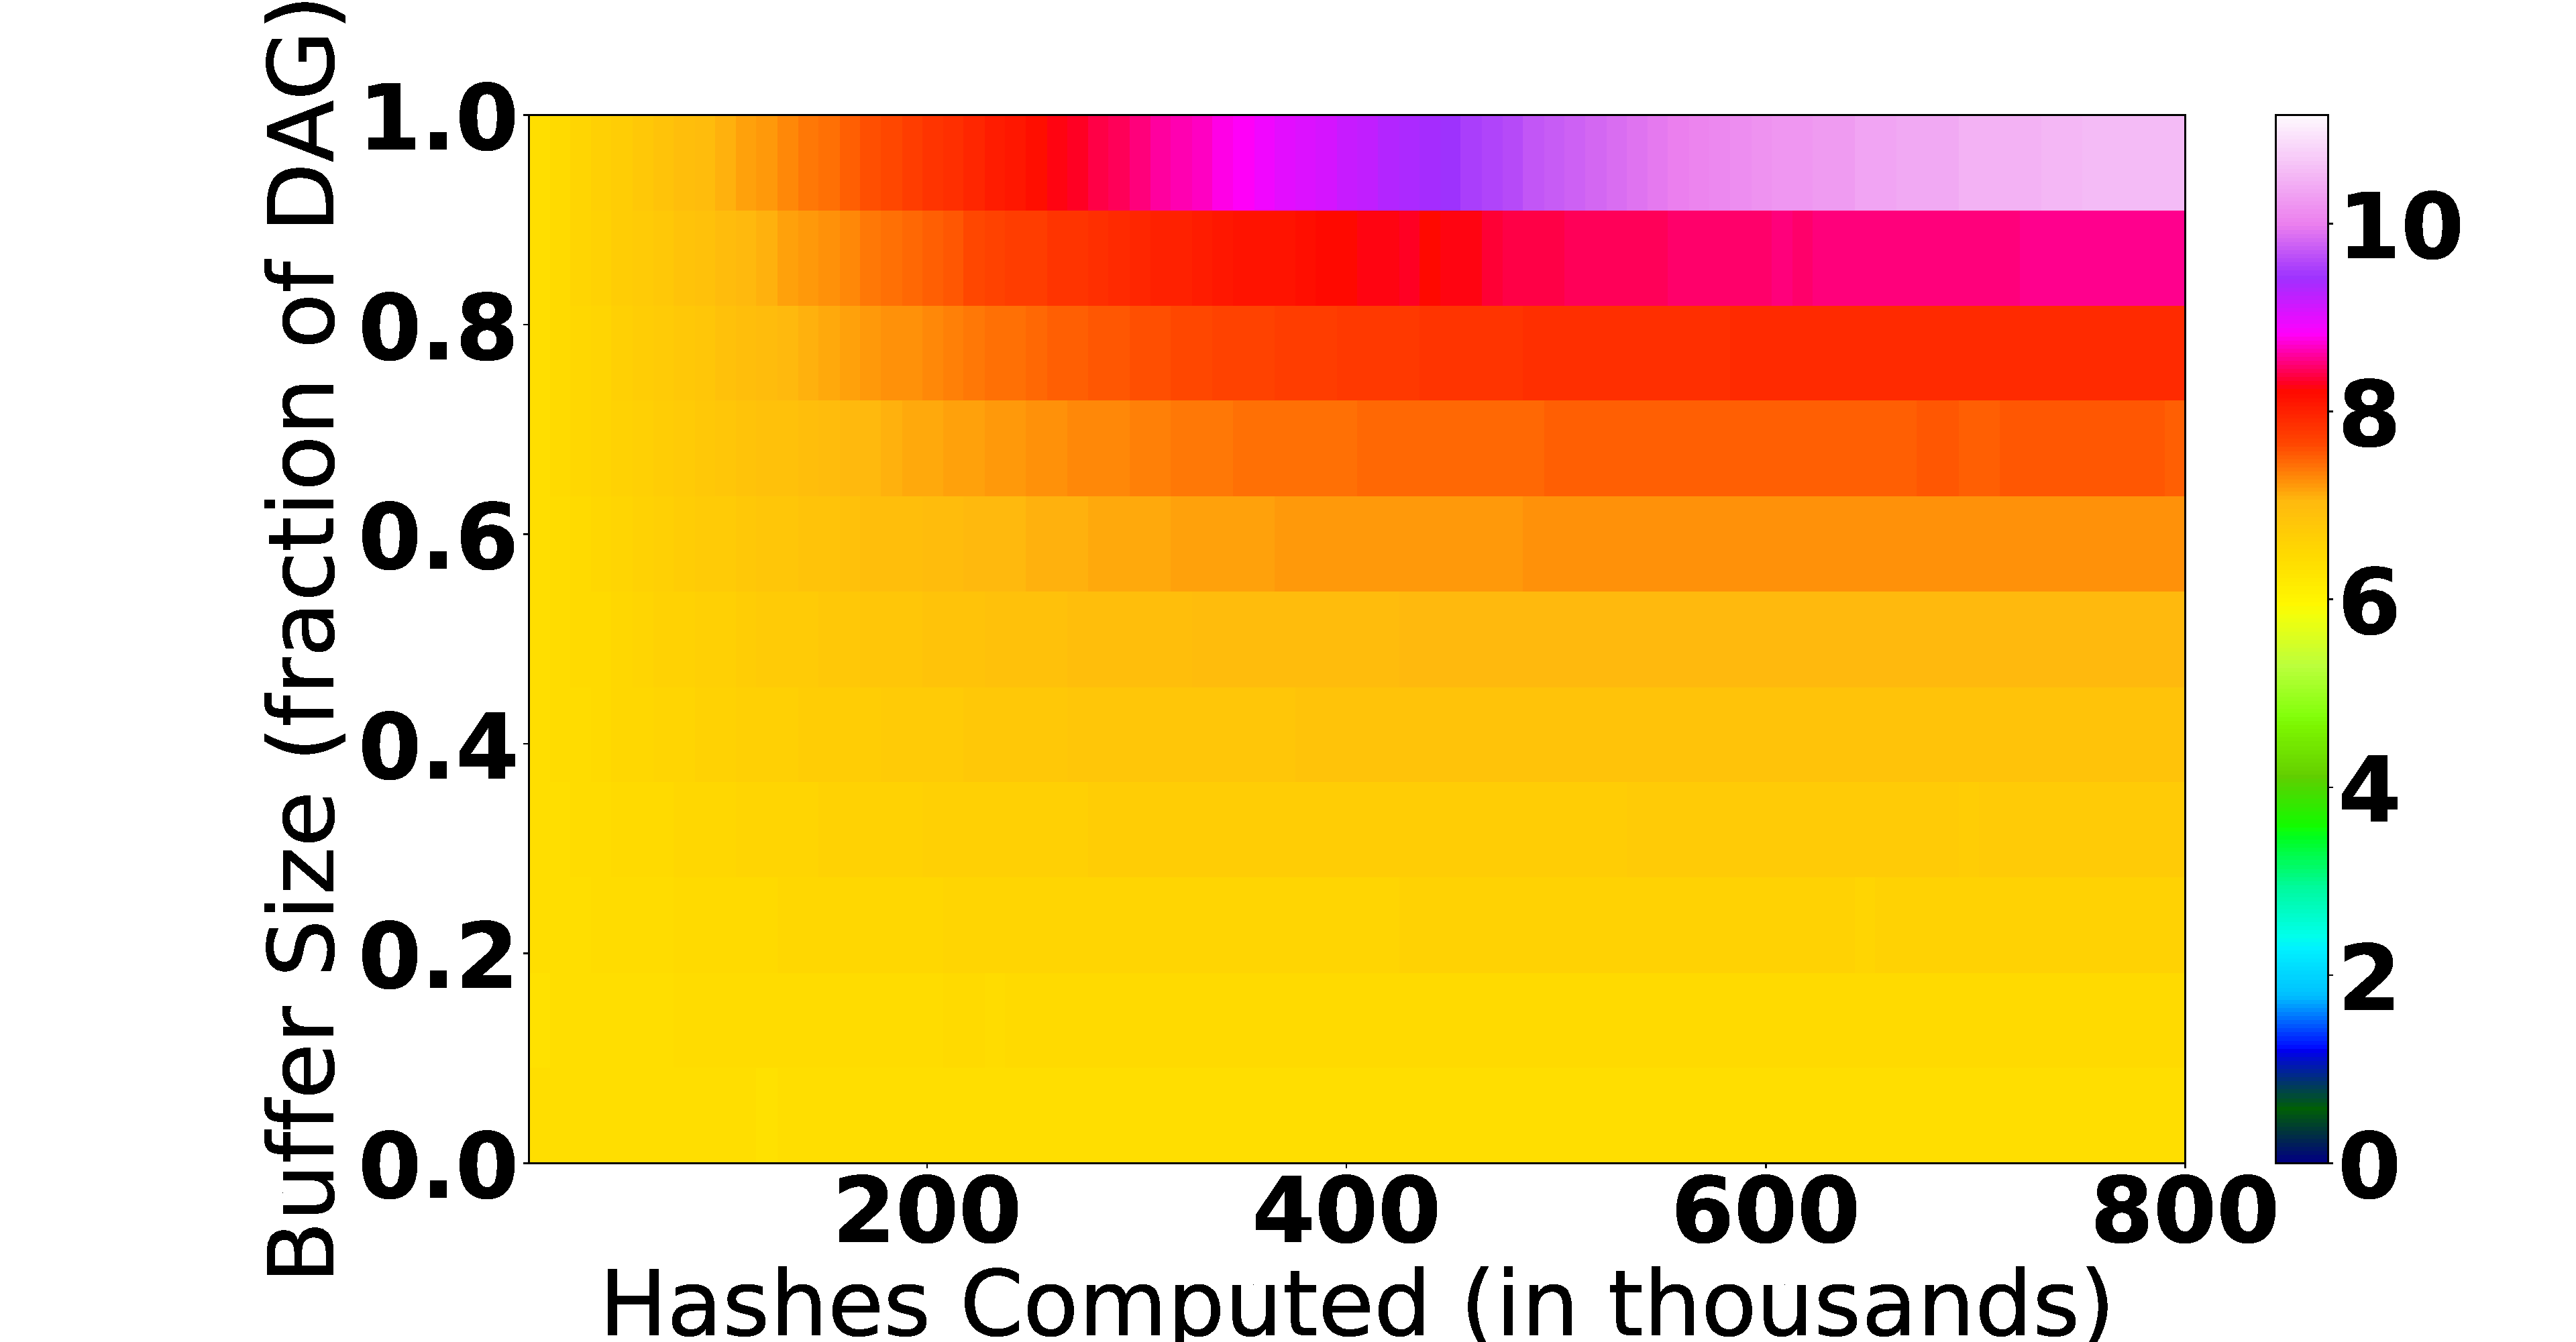
\includegraphics[width=\linewidth]{WebAssembly_Miner_Hash_Rate_HM.pdf}
\caption{WASM Miner $\log(Hash Rate)$}
\label{fig:hashRateHMWASM}
   \end{minipage}
       \begin{minipage}{.5\textwidth}
       \centering
    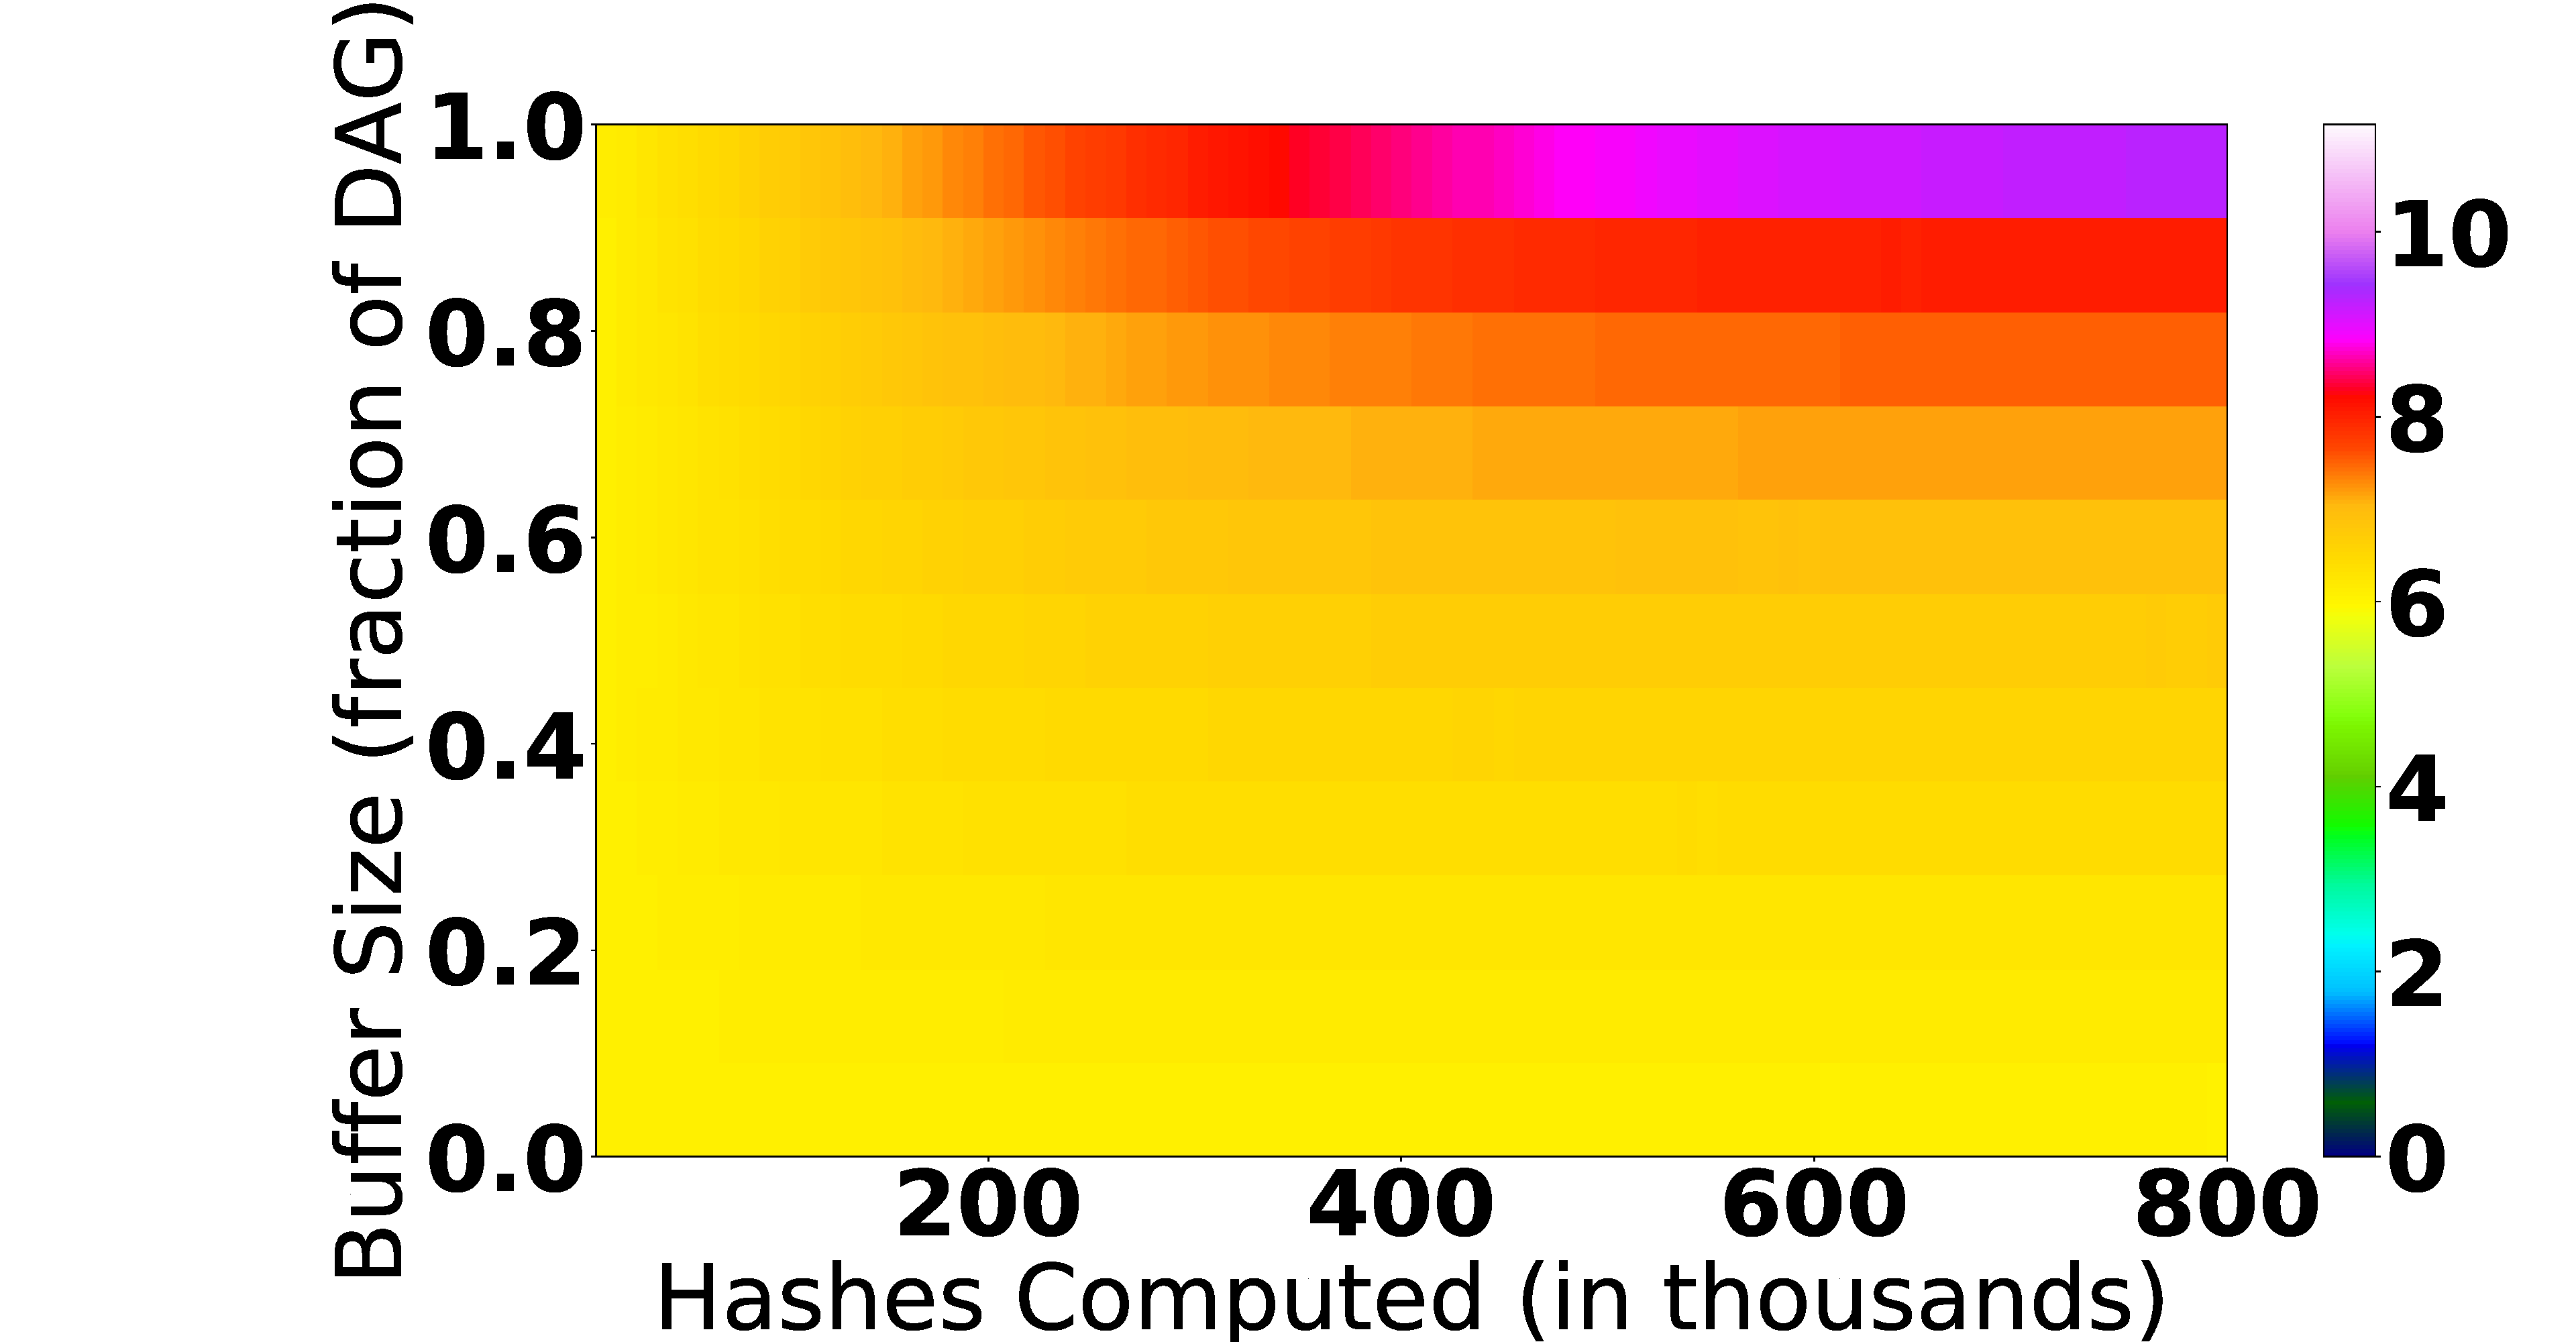
\includegraphics[width=\linewidth]{JavaScript_Miner_Hash_Rate_HM.pdf}
\caption{JS Miner $\log(Hash Rate)$}
\label{fig:hashRateHMJS}
    \end{minipage}}
\end{figure}

In order to closely examine the relationship between the hash rate and the hit rate, we show the correlations between the two parameters for all 3 miners in Figure \ref{fig:HashRateTraj}. It is interesting to see how the hash rate drastically spikes after the hit rate surpasses 95\%. This suggests that accessing DAG pages from the buffer is orders of magnitude faster than computing them, so much so that even a few computations bring down the hash rate drastically. Most importantly, from the experiments, the time it takes to reach this steady state hash rate is not long (about 5 minutes) thereby making this approach ideal for streaming/gaming websites. Furthermore, \verb|WebEth| is also ideal as a web miner as it is not very resource intensive -- throughout the experiments, it did not use more than 12.5\% of the CPU of our testing machine (the utilization value is normalized over 8 cores).

One might think that a way to reach the steady state hash rate faster for a given sized buffer would be to start out with a partially filled out buffer instead of an empty one. The only way this could work is by sending over part of the DAG over the network to the client. However, as it turns out, this is not feasible since, for a DAG with 16777186 nodes (1.074~GB) sending even 10\% of the DAG would be sending roughly 100~MB of data. With the global average download speed for desktops and smart phones being around 5.34~MBps and 2.77~MBps respectively~\cite{internetSpeed}, the web page load time would be in the order of 20 seconds to a minute -- which is too long to get a mere 10\% boost in the buffer storage. 

\begin{figure}[t]
\captionsetup{justification=centering}
       \centering
    \makebox[\textwidth][c]{
    \begin{minipage}{.5\textwidth}
       \centering
  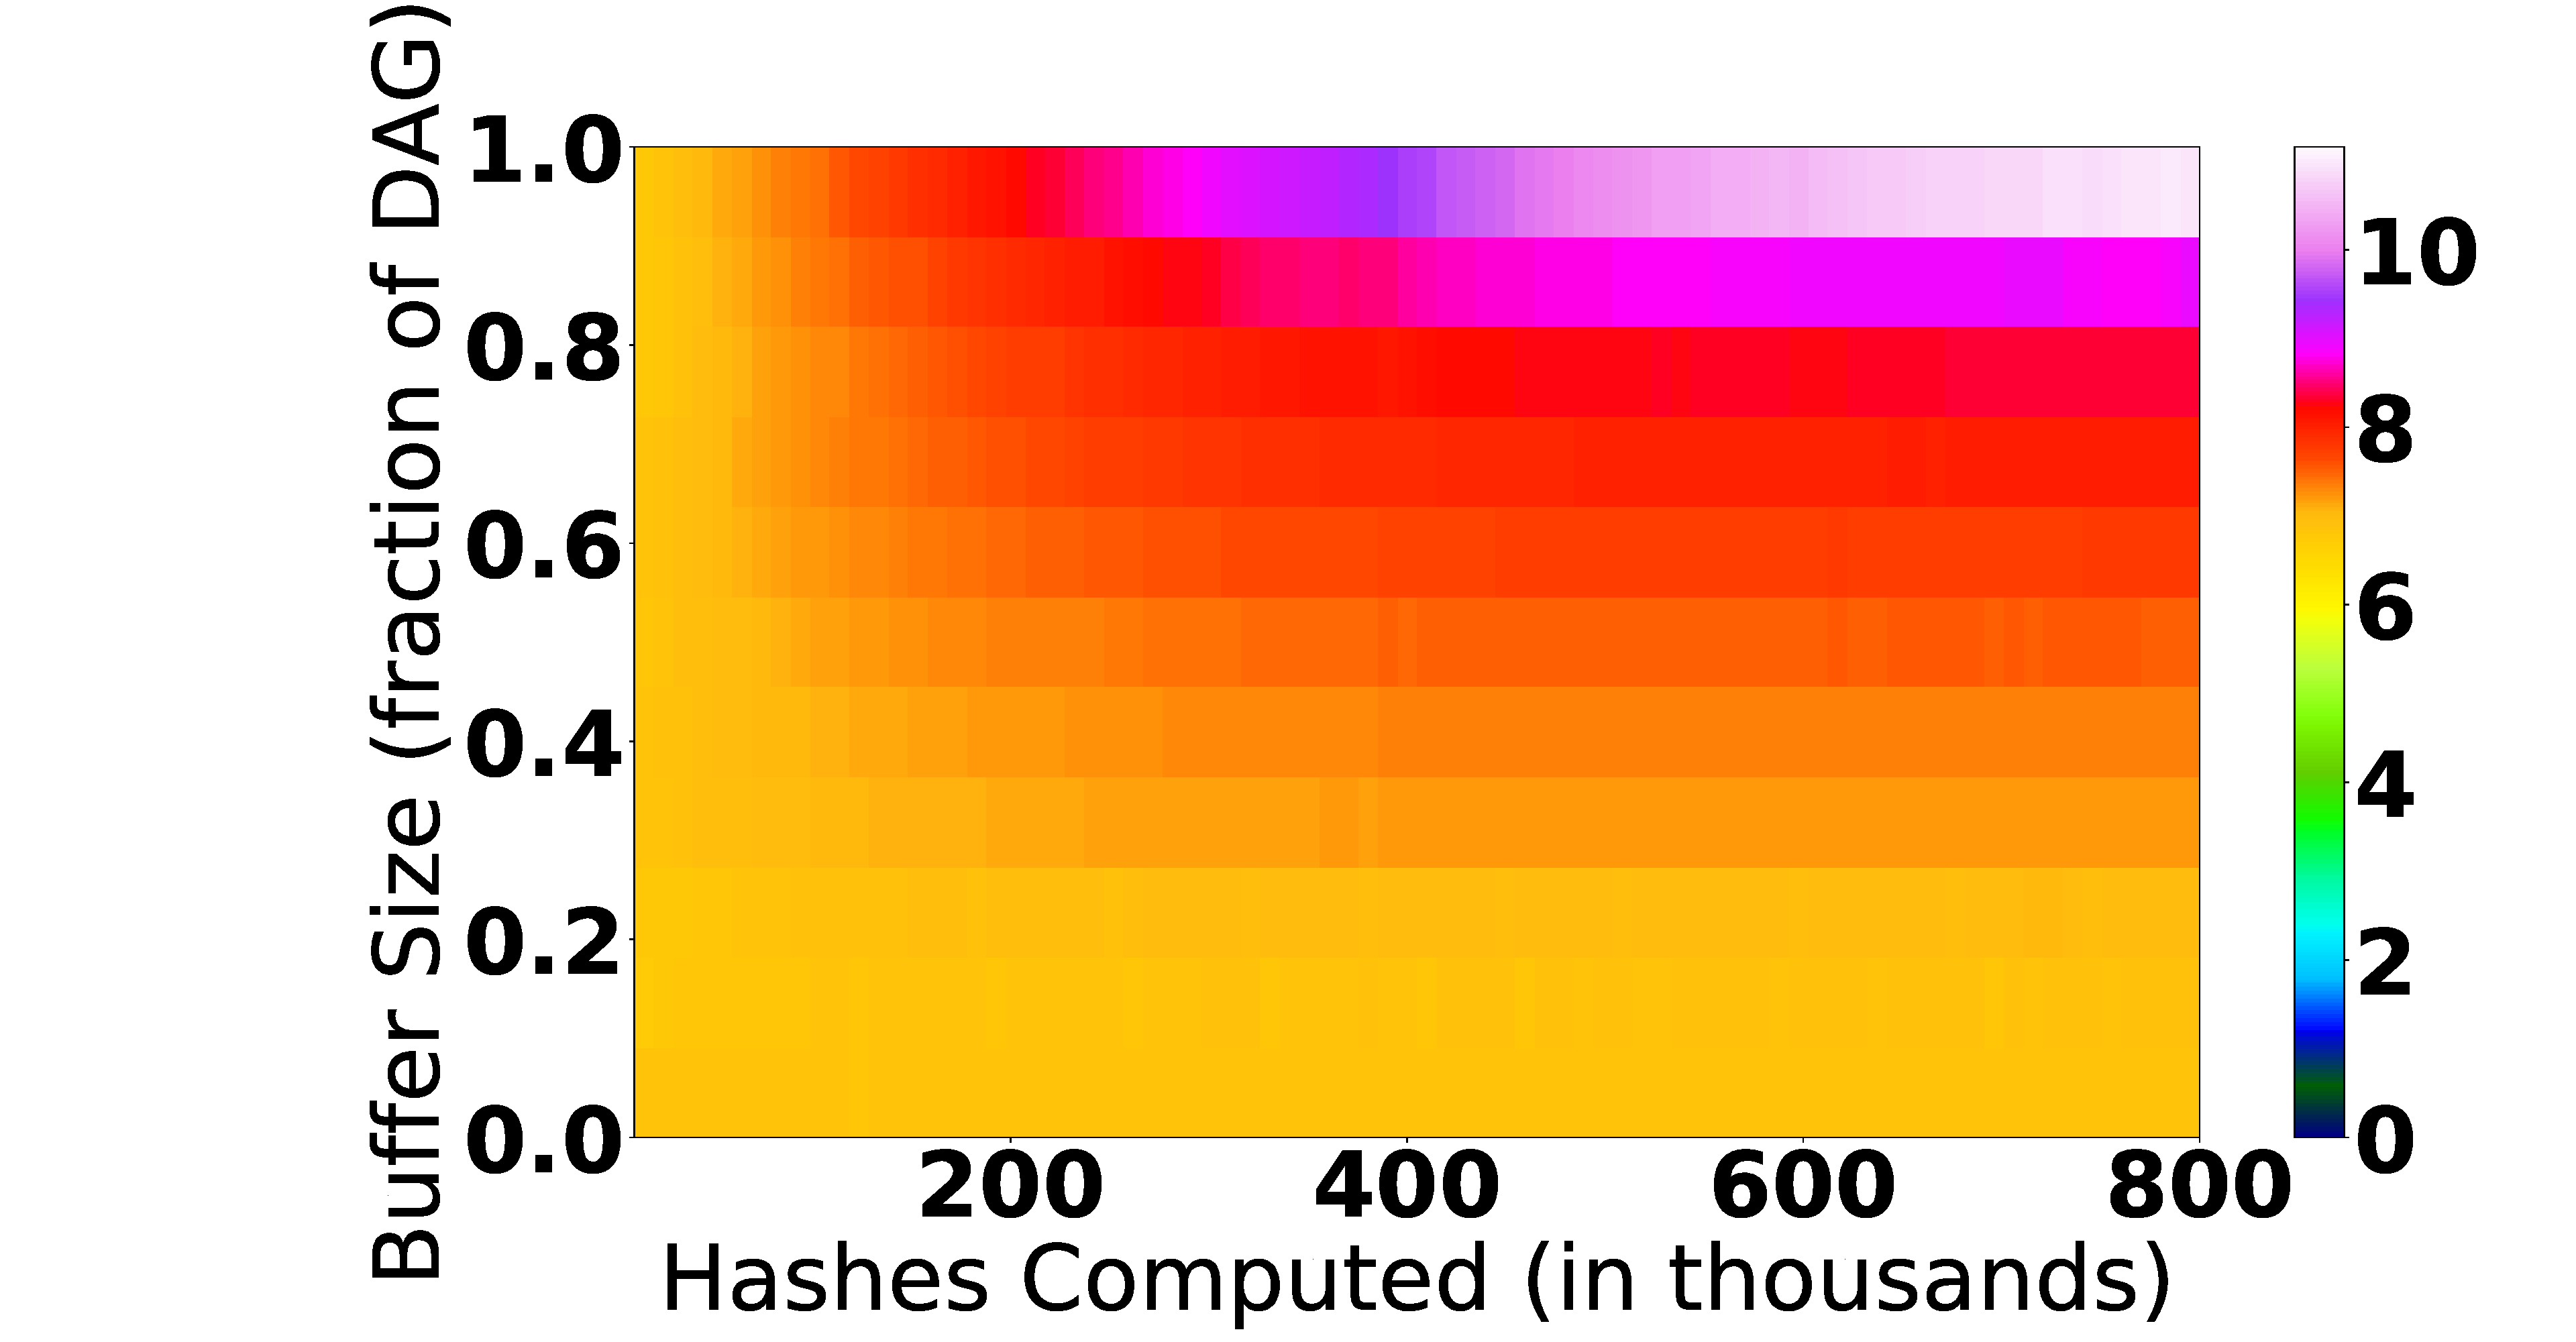
\includegraphics[width=\linewidth]{Native_C++_Miner_Hash_Rate_HM.pdf}
  \caption{Native C++ Miner $\log(Hash Rate)$}
  \label{fig:hashRateHMNative}
   \end{minipage}
       \begin{minipage}{.5\textwidth}
       \centering
    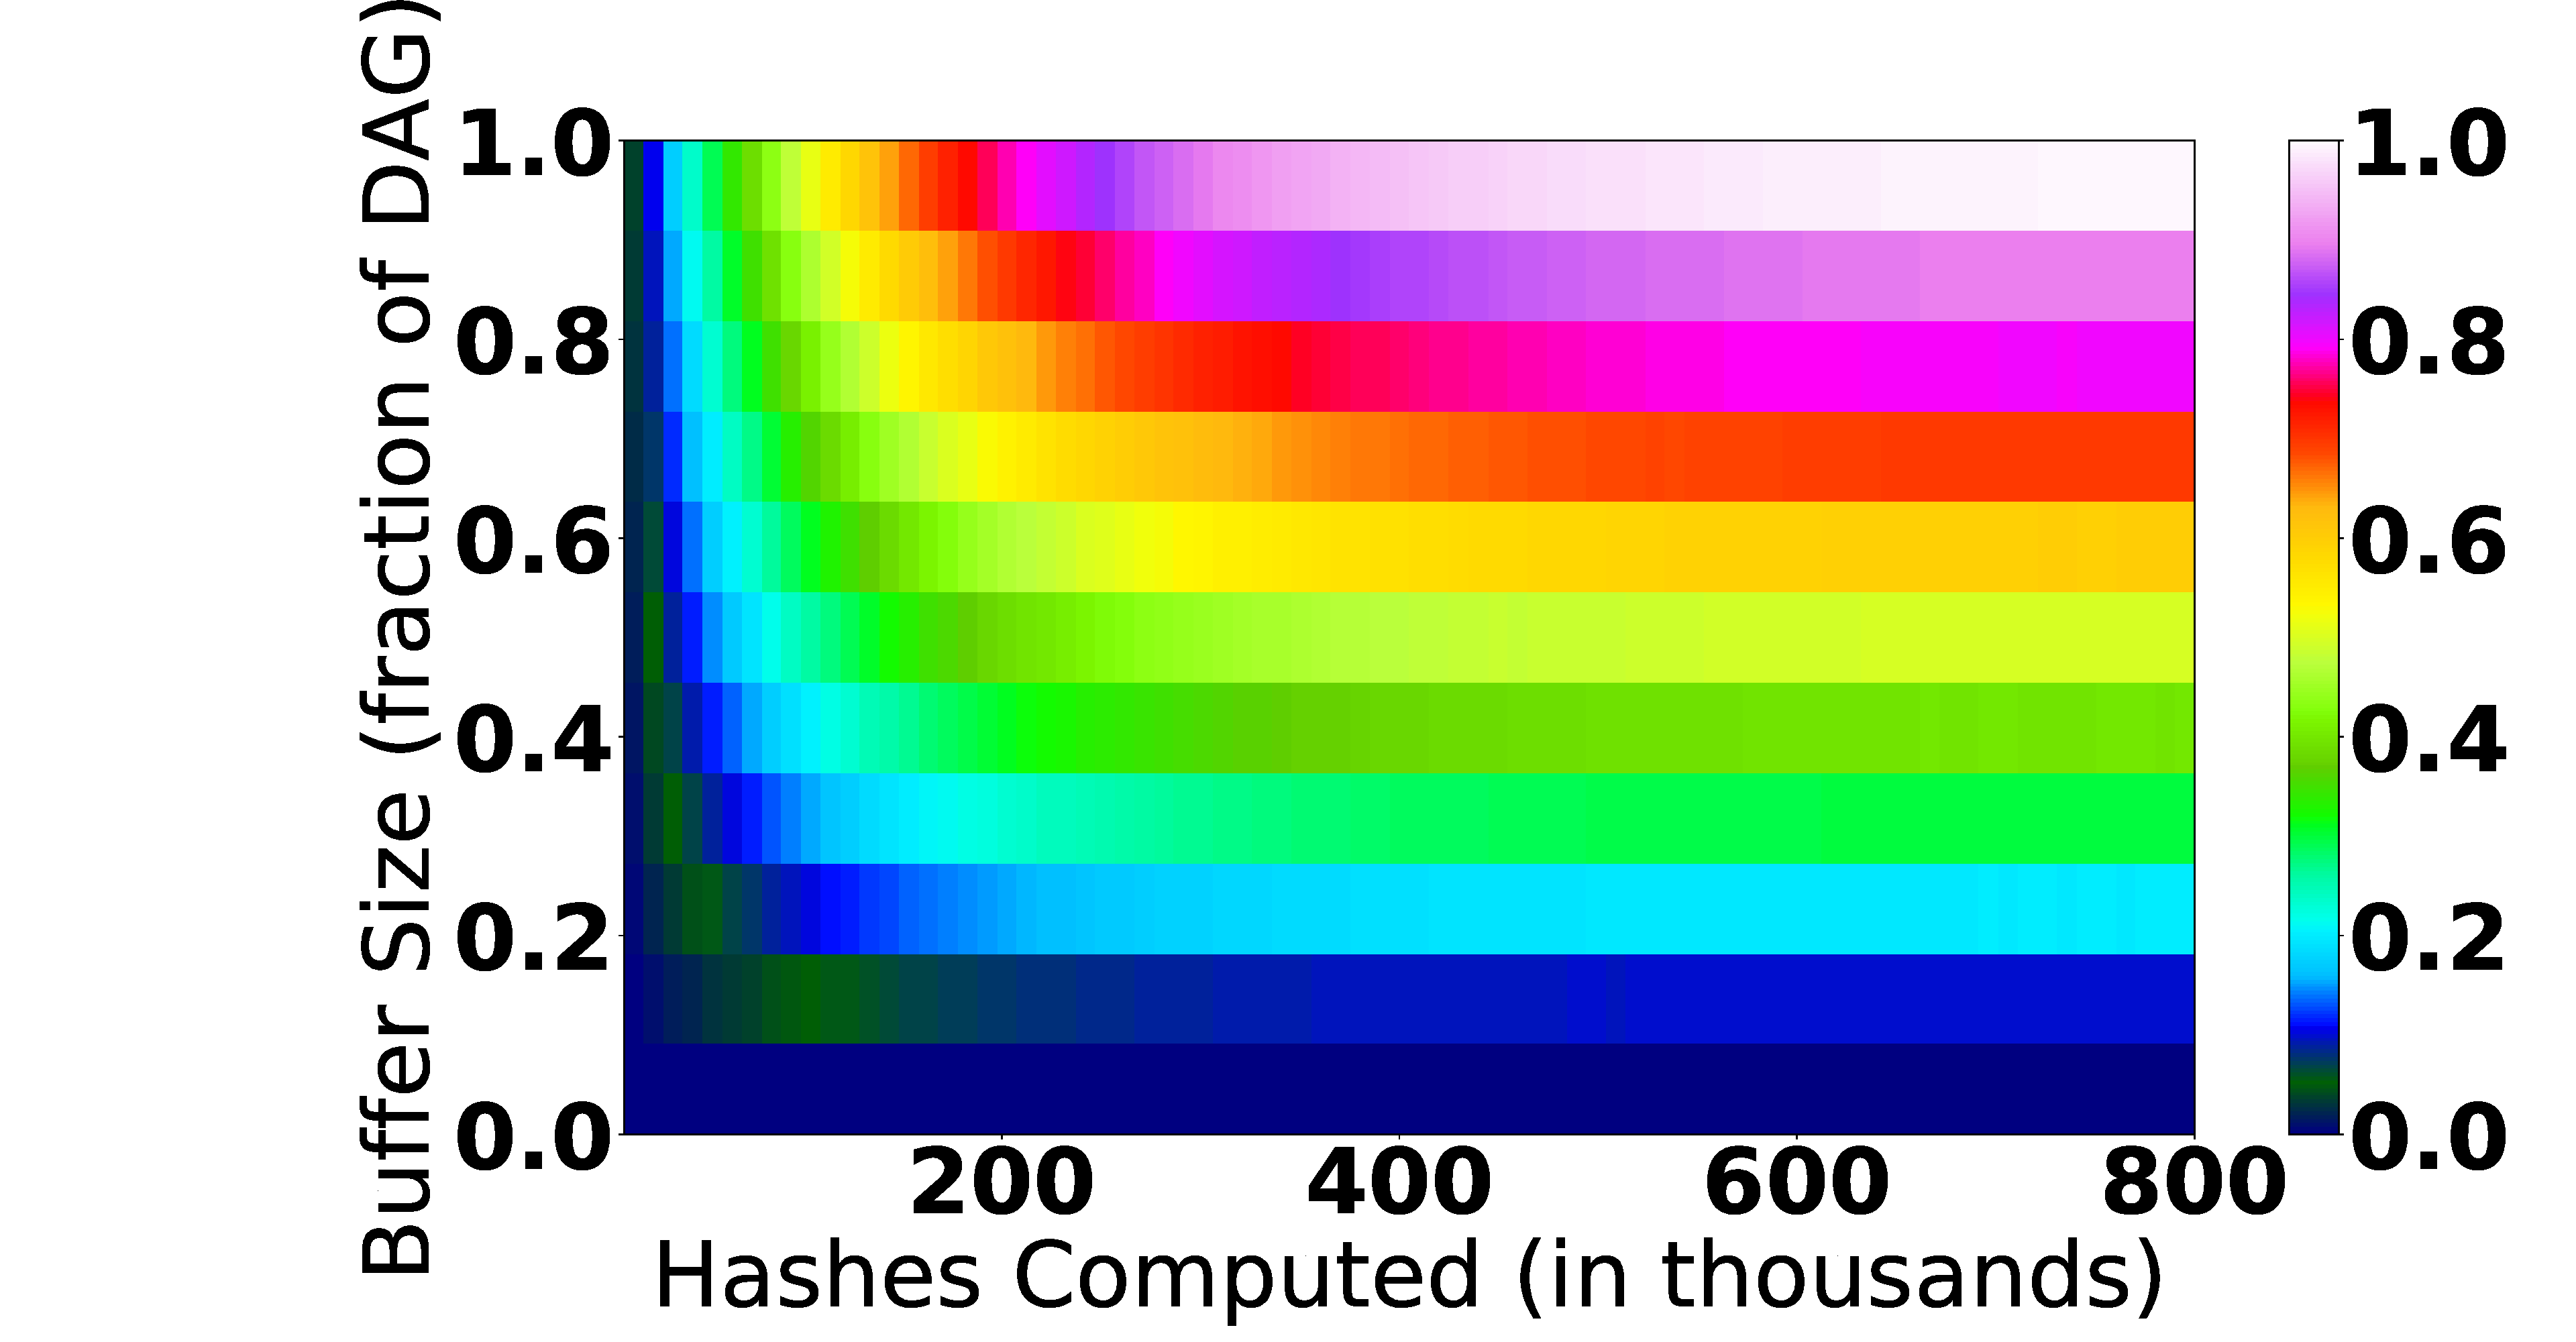
\includegraphics[width=\linewidth]{All_Miners_Buffer_Hit_Rate.pdf}
    \caption{All Miners' Hit Rate}
    \label{fig:HitRateHM}
    \end{minipage}}
\end{figure}
% Log(Hash Rate) and Hit Rate as a function of number of Hashes computed and Buffer Size

Table \ref{table:perf} shows us how the performance of each of the miners compare. Interestingly, the performance variation between different implementations is not uniform across different buffer sizes and hit rates. For instance, the variation between the \verb|WebAssembly| and \verb|JavaScript| miners is only 35.9\% when the buffer hit rate is 0, but the performance difference increases to 73.2\% when the hit rate becomes greater than 0.99. We also see that for obvious reasons, the native miner outperforms both the \verb|JavaScript| and the \verb|WebAssembly| miner. However, the \verb|WebAssembly| miner is at most 40.5\% slower than the native miner -- which is not very far off considering the overhead of running programs within browsers. The \verb|JavaScript| miner, on the other hand, is \textbf{at least} 47.2\% slower (and at most 82.0\% slower), making \verb|WebAssembly| the better of the two candidates for \verb|WebEth|.

\begin{table}[t]
\caption{Performance variations across different Implementations}\label{table:perf}
\vspace{-2ex}
\begin{center}
\begin{tabular}{ l  c  c  c}

&\makecell{\textbf{WASM/JS}} & \makecell{\textbf{Native/JS}} & \makecell{\textbf{Native/WASM}}\\
\cline{2\ -2} \cline{3\ -3} \cline{4\ -4}
\% Diff in smallest hash rates & 35.9\% &  55.0\% & 38.9\% \\
\% Diff in peak hash rates & 73.2\% &  81.3\% & 30.2\% \\
Min perf \% diff &  24.4\% &  47.2\% & 23.9\% \\
Max perf \% diff  &  73.3\% &  82.0\% & 40.5\%\\ 
Avg. Hash Rate \% diff\\
\qquad  (averaged over all buffer sizes\\
\qquad  and buffer hit rates)&  30.6\% &  55.6\% & 35.9\%\\
\end{tabular}
\end{center}
\vspace{-3ex}
\end{table}


Finally, we tabulate the most important results from our analysis in Table \ref{table:results}. We see that it takes all miners only a few hundred seconds to fill the buffer up, which is good considering the fact that most users don't stay on a particular website for very long. Furthermore, we see that the \verb|WebAssembly| miner is the better of the two miners, since it gives a better terminal hash rate of 40~kH/s.

\begin{table}[t]
\caption{Main Results}\label{table:results}
\vspace{-2ex}
\begin{center}
\begin{tabular}{ l  c  c  c}

&\makecell{\textbf{Native}} & \makecell{\textbf{JavaScript}} & \makecell{\textbf{WebAssembly}}\\
\cline{2\ -2} \cline{3\ -3} \cline{4\ -4}
\makecell[l]{Median Hash Rate \\
\qquad(for a buffer the size of the DAG)} & 15278~H/s &  5290~H/s & 10504~H/s \\
Peak Hash Rate &  56800~H/s &  10626~H/s & 39651~H/s \\
\makecell[l]{Time taken to 99.76\% \\ buffer hit rate}  &  163.601~s &  879.857~s & 257.7692~s\\ 
\makecell[l]{Avg. Hash Rate \% diff with Native Miner \\
\qquad(averaged over all buffer sizes)}&  NA &  55.6\% & 35.9\%\\
\end{tabular}
\end{center}
\vspace{-3ex}
\end{table}

\section{Potential Applications}
\label{sec:applications}
We envision that \verb|WebEth| could be used for a variety of applications.
\paragraph{Web Content Monetization:}
With the growth in global Internet usage, hosting websites has become a lucrative business. As a result, new methods of monetizing electronic content have surfaced with time. Though some are more successful than others, all of them have associated issues. For instance, selling advertisement space is now resulting in declining revenue for website owners due to the advent of new technologies such as AdBlock \cite{Adblock}, Brave Browser \cite{BraveBrowser,decliningRevenue}; when coupled with an increased load time, browser slow-down, and placement challenges, online ads adversely affect user experience.  Thus, we envision that website content can be monetized through client-size coin mining, utilizing techniques such as those presented in this work. Note though that earning real cash requires a significant subscriber base or a large amount of time spent on the website, making this an ideal approach for video streaming/gaming websites. In fact, with a hash rate of 40~kH/s, a website would need to have around 8000 users at any given time in order to obtain around \$500 per month \cite{etherProfit}.

\paragraph{Web Authentication Rate Limiting:}
Another potential application relates to rate limiting of web-authentication. Many tools are openly available for brute forcing web login pages~\cite{hydra,burpsuite}. Currently, the way website owners mitigate these attacks is by locking out a user for a certain amount of time after a fixed number of unsuccessful login attempts or presenting a captcha~\cite{recaptcha}.  
Lock out presents a Denial of Service potential by locking out legitimate users as a consequence of an attack. 
Captcha techniques can be used for third-party value~\cite{von2008recaptcha} and have been successfully attacked through machine learning techniques~\cite{mlCaptcha} and crowdsourcing~\cite{captchaFarms}. 
   
We posit a more user-friendly approach to this problem involving embedding a Proof-of-Work computation in a web page, \emph{e.g.}, using \verb|WebEth|, that the user's browser needs to successfully solve in order to be able to login. The PoW would amplify the computational power needed for brute force attempts, thereby selectively thwarting any attacker that attempts to brute force the login \emph{without} significantly penalizing the legitimate user. \verb|WebEth| is an especially good candidate for such an implementation because one could manually set the difficulty to obtain a balance between user experience and security.

\paragraph{Proof of Web Traffic:}
Another use-case of \verb|WebEth| involves website advertisement companies. Today, website advertising sponsors decide on the remuneration for a website based on summarized server logs as a measure for site traffic. These logs can be manipulated by a website owner to generate the impression of a large amount of traffic ~\cite{webLogsManipulation} or by ad injectors~\cite{adinjection}. As a solution to this, \verb|WebEth| could be embedded by a website owner within the website, thereby making the site visitors compute PoW hashes. The advertiser would then ask the website owner to submit hashes that pass a certain difficulty threshold (i.e., the value of the hash being less than a certain number), and the larger the number of hashes that the website owner can provide, the more the remuneration the site receives. This would be more difficult for the website owners to fake since they would have to compute hashes themselves, an endeavor that might be more expensive than the potential ad payout.

\paragraph{Private Ethereum Test Networks:}
Finally, we would also like to note that Ethereum is an extremely flexible currency in the sense that it allows for private coin networks -- \emph{i.e.,} networks that do not mine the public Ethereum block-chain, but rather a private (and often smaller) instance of the cryptocurrency. \verb|WebEth| can be used on any such private network to serve the network owner's specific interests.

\section{Conclusion}
\label{sec:conclusion}
We have designed and implemented \verb|WebEth|, an open-source and  distributed web-based Ethereum miner, with potential applications toward monetizing electronic content, rate limiting, private test networks, user tracking for advertisers, and the like. \verb|WebEth| is standalone, implemented in both \verb|JavaScript| and \verb|WebAssembly|, and requires no external dependencies, meaning that both of these implementations can be readily embedded within many existing websites.  We have also provided analyses and experimental data to help in engineering our proposed applications.

\paragraph{Future Work:}
Many interesting issues remain open.  For one, our current implementation is still slower than traditional mining methods. One way to speed this process up is to tap into the client machine's GPU. There is a \verb|JavaScript| library called WebCL that binds to the OpenCL library which allows \verb|JavaScript| to interact directly with the GPU to achieve better parallel performance. Knowing that Ethereum was created for GPU mining, it should provide a substantial improvement. 

Another interesting issue is whether the server should notify the clients once a new valid hash is found. One may expect that with a sufficiently large number of clients, this may lead to better performance than waiting for a timeout. In fact, experimenting with the length of the period before timeout might also be an interesting avenue to pursue.

The Ethereum Foundation is also currently developing Casper, a Proof-of-Stake algorithm, which has already been deployed in private testnets. Since Casper is open-source, it should be possible to create a Proof-of-Stake distributed browser miner implementation. However, users would most likely have to provide ``stakes" in order for such an implementation to be possible ~\cite{PoSproof}. Further research will be necessary to determine whether browser mining for Casper is viable or not, as the final form of Casper is still uncertain and exactly how much ``stake'' is required to successfully mine is unknown.

\section*{Acknowledgment}
The authors would like to thank Dennis Your for his contributions during the early stages of this research. This research was supported in part by NSF under grant CCF-1563753. Any
opinions, findings, and conclusions or recommendations expressed in this material
are those of the authors and do not necessarily reflect the views of the
NSF.

\begin{thebibliography}{1}
\bibitem{WebEth} Tiwari, Trishita, et al. ``WebEth.'' GitHub, 1.0, GitHub, 10 Apr. 2018, github.com/trishutiwari/web-ethereum-mining.

\bibitem{Adblock} Gundlach, Micheal. AdBlock browser extension. AdBlock. Software, 2009.

\bibitem{ethash}Matthew Wampler, et al. Ethash. Computer software. GitHub. Vers. 23.1. GitHub, 11 Jan. 2015. Web. 24 Feb. 2018. https://github.com/ethereum/ethash. 

\bibitem{BraveBrowser} Eich, Brendan and Brian Bondy. Brave Browser. Brave Software. Software, 2015.

\bibitem{decliningRevenue} Hern, Alex. ``Adblock Plus: the Tiny Plugin Threatening the Internet's Business Model.'' The Guardian, Guardian News and Media, 14 Oct. 2013, www.theguardian.com/technology/2013/oct/14/the-tiny-german-company-threatening-the-internets-business-model.

\bibitem{dagger-hashimoto} Buterin, Vitalik, et al. ``Ethereum/Wiki.'' GitHub, GitHub, 9 Feb. 2014, github.com/ethereum/wiki/blob/master/Dagger-Hashimoto.md. 

\bibitem{noSubscriptions} Rosenwald, Micheal. ``Digital News Consumers Unlikely to Pay for Content and Increasingly Block Ads.'' Columbia Journalism Review, Columbia Journalism Review, 15 June 2015, www.cjr.org/analysis/reuters\_digital\_news\_report.php.

\bibitem{payPerClick} Fessenden, Therese. ``Nielsen Norman Group.'' The Most Hated Online Advertising Techniques, Nielsen Norman Group, 4 June 2017, www.nngroup.com/articles/most-hated-advertising-techniques/.

\bibitem{celebEndorse} Awad, Amal. ``A Study in Scarlett: The Ethics of Celebrity Endorsement.'' – Opinion – ABC Religion \&Amp; Ethics (Australian Broadcasting Corporation), Amal Awad ABC Religion and Ethics, 30 Jan. 2014, www.abc.net.au/religion/articles/2014/01/31/3935443.htm.

\bibitem{scheduling}
Ramamritham, Krithi, and John A. Stankovic. ``Dynamic task scheduling in hard real-time distributed systems.'' IEEE software 1.3 (1984): 65.

\bibitem{parallel}
Shirazi, Behrooz A., Krishna M. Kavi, and Ali R. Hurson. Scheduling and load balancing in parallel and distributed systems. IEEE Computer Society Press, 1995.

\bibitem{orca}
Bal, Henri E., M. Frans Kaashoek, and Andrew S. Tanenbaum. ``Orca: A language for parallel programming of distributed systems.'' IEEE transactions on software engineering 18.3 (1992): 190-205.

\bibitem{WebFlow}
Bhatia, Dimple; Burzevski, Vanco; Camuseva, Maja; and Fox, Geoffrey C., ``WebFlow - A Visual Programming Paradigm for Web/Java Based Coarse Grain Distributed Computing'' (1997).
Northeast Parallel Architecture Center.

\bibitem{Cushing} Cushing, Reginald, et al. ``Distributed Computing on an Ensemble of Browsers.'' IEEE Internet Computing, IEEE, 1 Sept. 2013, www.computer.org/csdl/mags/ic/2013/05/mic2013050054.html.

\bibitem{randmemohash} Lerner, Sergio Demian. ``Strict Memory Hard Hashing Functions (Preliminary V0. 3, 01-19-14)."

\bibitem{coinhive}
The Coinhive Team. Coinhive browser extension. Coinhive. Software, 2017.

\bibitem{pow}
Laurie, Ben, and Richard Clayton. ``Proof-of-work proves not to work; version 0.2.'' Workshop on Economics and Information, Security. 2004.

\bibitem{casper}
Hertig, Alyssa. ``Ethereum's Big Switch: The New Roadmap to Proof-of-Stake.'' CoinDesk, CoinDesk, 16 May 2017, www.coindesk.com/ethereums-big-switch-the-new-roadmap-to-proof-of-stake/. 

\bibitem{pos}
Dmitry Buterin, et al. ``Proof of Work vs Proof of Stake: Basic Mining Guide.'' Blockgeeks, Blockgeeks, 24 July 2017, blockgeeks.com/guides/proof-of-work-vs-proof-of-stake/. 

\bibitem{Monero} ``Monero - Secure, Private, Untraceable.'' Getmonero.org, The Monero Project, getmonero.org/.

\bibitem{Duda} Duda, Jerzy, and Wojciech Dłubacz. ``Distributed Evolutionary Computing System Based on Web Browsers with Javascript.'' ACM Digital Library, Springer-Verlag, dl.acm.org/citation.cfm?id=2451764.2451780.

\bibitem{traffic} The SimilarWeb Team. SimilarWeb LTD 2017. (https://www.similarweb.com/)

\bibitem{coinwarz}Coinwarz Ethereum Mining Calculator and Profit Calculator. Coinwarz 2017. (https://www.coinwarz.com/calculators/ethereum-mining-calculator)

\bibitem{PoSproof}Dale, Oliver. ``Beginner's Guide to Ethereum Casper Hardfork: What You Need to Know''. Blocknomi, 7 November 2017. (https://blockonomi.com/ethereum-casper/)

\bibitem{Ethmining}
Wood, Gavin. ``Ethereum: A secure decentralised generalised transaction ledger.'' Ethereum Project Yellow Paper 151 (2014): 1-32.

\bibitem{geth}Péter Szilágyi, et al. Geth. Computer software. GitHub. Vers. 1.8.1. GitHub, 22 Dec. 2013. Web. 24 Feb. 2018. https://github.com/ethereum/go-ethereum. 

\bibitem{etherscan}Etherscan The Ethereum Block Explorer. Etherscan 2017. (https://etherscan.io/charts)

\bibitem{remote} remoteStorage: An open protocol for per-user storage on the Web. (https://remotestorage.io/)

\bibitem{webAssembly}  W3C Team. WebAssembly. Program documentation. WebAssembly. Vers. 1.0. WebAssembly, 17 Mar. 2017. Web. 28 Mar. 2018. http://webassembly.org. 

\bibitem{wasmPerf} Zlatkov, Alexander. ``How JavaScript Works: A Comparison with WebAssembly.'' SessionStack Blog. SessionStack Blog, 21 Nov. 2017. Web. 28 Mar. 2018. https://blog.sessionstack.com/how-javascript-works-a-comparison-with-webassembly-why-in-certain-cases-its-better-to-use-it-d80945172d79. 

\bibitem{emscripten} Emscripten Community. Emscripten. Emscripten. Vers. 1.37.36. Emscripten, 11 Nov. 2012. Web. 28 Mar. 2018. http://kripken.github.io/emscripten\-site/docs/getting\_started/Tutorial.html. 

\bibitem{internetSpeed} Ookla. ``Speedtest Global Index – Monthly Comparisons of Internet Speeds from around the World.'' Speedtest Global Index, Ookla, 25 Mar. 2018, www.speedtest.net/global-index.

\bibitem{hydra}  Fogerlie, Garrett, director. Brute Force Website Login Attack Using Hydra - Hack Websites - Cyber Security. Brute Force Website Login Attack Using Hydra - Hack Websites - Cyber Security, YouTube, 24 Sept. 2013, www.youtube.com/watch?v=ZVngjGp-oZo. 

\bibitem{burpsuite} Mahmood, Osama. ``Brute Force Website Login Page Using Burpsuite –.'' SecurityTraning, SecurityTraning, 5 Feb. 2018, securitytraning.com/brute-force-website-login-page-using-burpsuite/. 

\bibitem{webLogsManipulation} Fox\-Brewster, Thomas. ``'Biggest Ad Fraud Ever': Hackers Make \$5M A Day By Faking 300M Video Views.'' Forbes, Forbes Magazine, 20 Dec. 2016, www.forbes.com/sites/thomasbrewster/2016/12/20/methbot\-biggest\-ad\-fraud\-busted/\#73f089a94899/ 

\bibitem{couponCollector} Neal, Peter. ``The Generalised Coupon Collector Problem.'' Journal of Applied Probability, vol. 45, no. 3, 2008, pp. 621\-629., doi:10.1239/jap/1222441818.

% \bibitem{harmonicNumber} Guo, Bai-Ni \& Qi, Feng. (2011). Sharp bounds for harmonic numbers. Applied Mathematics and Computation. 218. 991-. 10.1016/j.amc.2011.01.089.

\bibitem{recaptcha} Google recaptcha, \url{https://www.google.com/recaptcha/intro/}.

\bibitem{von2008recaptcha} Von Ahn, Luis and Maurer, Benjamin and McMillen, Colin and Abraham, David and Blum, Manuel, ``Recaptcha: Human-based character recognition via web security measures'', Science, vol. 321, no. 5895, pp. 1465-1468, 2008.

\bibitem{adinjection} Thomas, Kurt, et al. ``Ad injection at scale: Assessing deceptive advertisement modifications.'' IEEE Symposium on Security and Privacy, 2015.

\bibitem{ethereum} ``Ethereum: A secure decentralised generalised transaction ledger''. G Wood. 2014. cryptopapers.net Ethereum Project Yellow Paper.

\bibitem{keccak} Bertoni, Guido, et al. ``Keccak.'' Annual International Conference on the Theory and Applications of Cryptographic Techniques. Springer, Berlin, Heidelberg, 2013.

\bibitem{asics} Taylor, Michael Bedford. ``The Evolution of Bitcoin Hardware.'' Computer 50.9 (2017): 58-66.

\bibitem{js} Peyrott, Sebastián. ``A Brief History of JavaScript.'' Auth0 - Blog, Auth0, 16 Jan. 2017, auth0.com/blog/a-brief-history-of-javascript/. 

\bibitem{basicAttentionToken} Brave Software. ``Basic Attention Token.'' Basic Attention Token, 1.0, Brave Software, 13 Mar. 2018, basicattentiontoken.org/. 

\bibitem{mlCaptcha} Geitgey, dam. ``How to Break a CAPTCHA System in 15 Minutes with Machine Learning.'' Medium, Medium, 13 Dec. 2017, medium.com/@ageitgey/how-to-break-a-captcha-system-in-15-minutes-with-machine-learning-dbebb035a710. 

\bibitem{captchaFarms} Danchev, Dancho. ``Inside India's CAPTCHA Solving Economy.'' ZDNet, ZDNet, 4 Dec. 2015, www.zdnet.com/article/inside-indias-captcha-solving-economy/.

\bibitem{erc20} ``ERC20 Token Standard,'' \\\url{https://theethereum.wiki/w/index.php/ERC20\_Token\_Standard}.

\bibitem{etherProfit} CryptoCompare. ``Mining Calculator Bitcoin, Ethereum, Litecoin, Dash and Monero.'' CryptoCompare, CryptoCompare, 
www.cryptocompare.com/mining/calculator/eth. 
\end{thebibliography}

\addtolength{\textheight}{-7cm}
% \balance


% that's all folks
\end{document}